The MiniMax algorithm is a decision rule algorithm for minimizing the possible
loss for a worst case (maximum loss) scenario in a zero sum game for 2 (or more)
players who play in turns.

The algorithm builds a game tree, where each tree node represents a game state
and the children represent the possible game moves that can be made by either
player 1 or player 2.  An evaluation function is used to compute the score of
the board for each leaf of the tree. A node is a leaf when the game state can no
longer be expanded. Finally, the algorithm recursively minimizes or maximizes
the scores of each node. To select the best move for player 1, the algorithm
picks the move maximized at the root node.

In LM, the program starts with a root node (with the initial game state) that
is expanded with the available moves at each level. The graph of the program is
dynamic since nodes are created and then deleted once they are no longer
needed. The latter happens when the leaf scores are computed or when a node
fully minimizes or maximizes the children scores. When the program ends, only
the root node has facts in its database.

The full MiniMax code is shown in Fig.~\ref{code:coord:minimax}. The first two
rules in lines~\ref{line:coord:minimax_play1}-\ref{line:coord:minimax_play2}
check if the current game is final, namely, if a player has won or the game
drew: the first rule generates the score for the final state while the second
expands the game state by generating all the possible plays for player
\code{NextPlayer}.

The expansion rules creates the children for the current node and are
implemented in
lines~\ref{line:coord:minimax_expand1}-\ref{line:coord:minimax_expand2}. The
first two rules create either a \code{maximize} or \code{minimize} fact that
will either maximize or minimize the scores of the children nodes.  The third
and fourth expansion rules simulate a player move and, for that, create a new
node \code{B} using the \code{exists} language construct. We link \code{B} with
\code{A} using \code{parent(B, A)} and kickstart the recursive expansion of node
\code{B} by deriving a \code{play} fact. Finally, the rule in
lines~\ref{line:coord:minimax_expand11}-\ref{line:coord:minimax_expand2} is for
the case when the current player cannot play in the current game position.

\begin{wrapfigure}{r}{0.4\textwidth}
   \begin{center}
      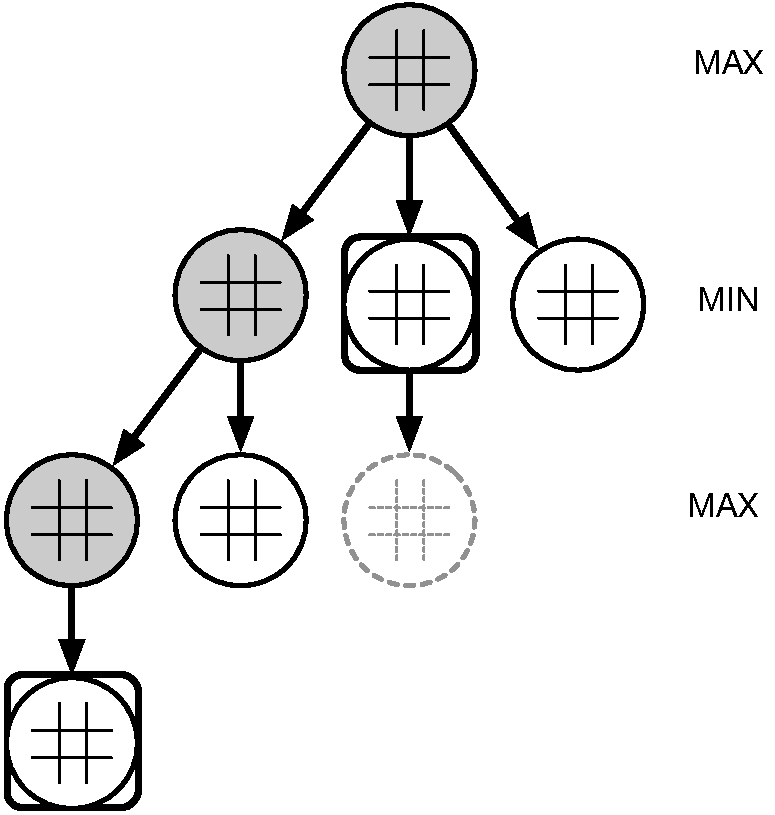
\includegraphics[width=0.9\linewidth]{figures/coordination/minimax_tree}
   \end{center}
   \caption{Expanding the MiniMax tree using coordination. By prioritizing
      deeper nodes, threads are forced to expand the tree using a depth-first
      approach, which is superior since there is no need to expand the whole
      tree before computing the node scores.}
   \label{fig:coord:minimax}
\end{wrapfigure}

As noted in Section~\ref{sec:coord:fifo}, the default scheduler uses a FIFO
approach, which results in a breadth-first search on the MiniMax tree. This
results in $\mathcal{O}(n)$ space complexity, where $n$ is the number of nodes
in the tree, since the tree must be fully expanded before the scores at the
leaves are actually computed.  With coordination, we set the priority of a node
to be its depth (lines~\ref{line:coord:minimax_coord1} and
\ref{line:coord:minimax_coord2}) so that the tree is expanded in a depth-first
fashion, leading to $\mathcal{O}(d t)$ memory complexity, where $d$ is the depth
of the tree and $t$ is the number of threads. Since threads prioritize deeper
nodes, the scores of the first leaves are immediately computed and then sent to
the parent node. At this point, the leaves are deleted and reused for other
nodes in the tree, resulting in minimal memory usage.  As an example, consider a
system with 2 threads, $T_1$ and $T_2$, where $T_1$ first expands the root node
and then the first child. Since $T_2$ is idle, it steals half of the root's
children nodes and starts expanding one of the nodes in a depth-first fashion.

\begin{figure}[ht]
\begin{Verbatim}[numbers=left,commandchars=\\\{\},fontsize=\codesize]
type list int game.
type linear parent(node, node).
type linear score(node, int, int). type linear new-score(node, int, int).
type linear minimize(node, int, int, int). type linear maximize(node, int, int, int).
type linear expand(node, game FirstPart, game SecondPart,
   int Descendants, int Player, int Play, int Depth).
type linear play(node, game Game, int Player, int Play, int Depth).

const root-player = 1. const initial-game = [...].
fun next(P : int) : int = if P = 1 then 2 else 1 end.

play(@0, initial-game, root-player, 0, 1).\label{line:coord:minimax_axiom}

play(A, Game, NextPlayer, LastPlay, Depth),\label{line:coord:minimax_play1}
Score = minimax_score(Game, NextPlayer, root-player), Score > 0
   -o score(A, Score, LastPlay).
play(A, Game, NextPlayer, LastPlay, Depth),
0 = minimax_score(Game, NextPlayer, root-player)
   -o expand(A, [], Game, 0, NextPlayer, LastPlay, Depth).\label{line:coord:minimax_play2}

expand(A, Game, [], N, Player, Play, \underline{Depth}), Player = root-player\label{line:coord:minimax_expand1}
  -o maximize(A, N, -00, 0).
expand(A, Game, [], N, Player, Play, \underline{Depth}), Player <> root-player
  -o minimize(A, N, +00, 0).
expand(A, First, [0 | Xs], N, Player, Play, \underline{Depth}), Depth >= 5
   -o exists B. (\underline{set-static(B)},\label{line:coord:minimax_coord1}
       \underline{set-default-priority(B, float(Depth + 1))},\label{line:coord:minimax_coord2}
       play(B, Game ++ [P | Xs], next(P), N, \underline{Depth + 1}), parent(B, A).
       expand(A, First ++ [0], Xs, N + 1, Player, Play, \underline{Depth})).
expand(A, First, [0 | Xs], N, Player, Play, \underline{Depth}), Depth < 5
  -o exists B. (\underline{set-default-priority(B, float(Depth + 1))},\label{line:coord:minimax_coord3}
       play(B, Game ++ [P | Xs], next(P), N, \underline{Depth + 1}), parent(B, A),
       expand(A, First ++ [0], Xs, N + 1, Player, Play, \underline{Depth})).
expand(A, First, [C | Xs], N, Player, Play, \underline{Depth}) C <> 0\label{line:coord:minimax_expand11}
  -o expand(A, First ++ [C], Xs, N, Player, Play, \underline{Depth}).\label{line:coord:minimax_expand2}

score(A, Score, BestPlay), parent(A, B) -o new-score(B, Score, BestPlay).\label{line:coord:minimax_new}

new-score(A, Score, Play), minimize(A, N, Current, BestPlay), Current > Score\label{line:coord:minimax_minimize1}
   -o minimize(A, N - 1, Score, Play).
new-score(A, Score, Play), minimize(A, N, Current, BestPlay), Current <= Score
   -o minimize(A, N - 1, Current, BestPlay).
minimize(A, 0, Score, BestPlay) -o score(A, Score, BestPlay).\label{line:coord:minimax_minimize2}

new-score(A, Score, Play), maximize(A, N, Current, BestPlay), Current < Score\label{line:coord:minimax_maximize1}
   -o maximize(A, N - 1, Score, Play).
new-score(A, Score, Play), minimize(A, N, Current, BestPlay), Current >= Score
   -o maximize(A, N - 1, Current, BestPlay).
maximize(A, 0, Score, BestPlay) -o score(A, Score, BestPlay).\label{line:coord:minimax_maximize2}
\end{Verbatim}
\caption{LM code for the MiniMax program.}
\label{code:coord:minimax}
\end{figure}

We also take advantage of memory locality by using \code{set-static}
(line~\ref{line:coord:minimax_coord2}), so that nodes after a certain level are
   not stolen by other threads. While this is not critical for performance in
   shared memory systems where node stealing is fairly efficient, we expect that
   such coordination to be critical in distributed systems.

The rest of the program contains rules for maximizing and minimizing scores
(lines~\ref{line:coord:minimax_minimize1}-\ref{line:coord:minimax_maximize2}),
through the retraction of \code{new-score} incoming facts.

\begin{figure}[ht]
   \begin{center}
      \begin{tabular}[b]{ | c | c | c |}
         \hline
         \textbf{\# T} & \textbf{Reg} & \textbf{Coord} \\ \hline \hline
         1 & 4.85GB & 0.38MB \\ \hline
         2 & 5.29GB & 0.65MB \\ \hline
         4 & 5.88GB & 1.28MB \\ \hline
         8 & 5.66GB & 2.42MB \\ \hline
         16 & 5.04GB & 4.68MB \\ \hline
         \end{tabular}
   \end{center}

   \caption{(a) Memory usage and (b) scalability of the regular and coordinated
versions of MiniMax.}
   \label{results:memory_minmax}
\end{figure}

In Fig.~\ref{results:memory_minmax} we compare the memory usage and scalability
of the coordinated MiniMax against the regular MiniMax. The coordinated version
uses significantly less memory (at most 4.68MB for 16 threads) than the regular
version (around 5.04GB). Note that as the number of threads goes up, memory
usage also goes up. This is an artifact of our parallel memory allocator that
allocates large chunks of memory beforehand. In terms of scalability, our
experimental results show that the coordinated version running on 16 threads is
almost 4 times faster than the hand-written sequential C program, while the
regular version is barely as fast as the same C program. XXX

\subsubsection{Proof Of Correctness}
